% LaTeX Template for Project Report, Version 2.0
% (Abstracted from a Major Project Report at CSED, NIT Calicut but can be
% modified easily to use for other reports also.)
%
% Released under Creative Commons Attribution license (CC-BY)
% Info: http://creativecommons.org/licenses/by/3.0/
%
% Created by: Kartik Singhal
% BTech CSE Batch of 2009-13
% NIT Calicut
% Contact Info: kartiksinghal@gmail.com
%
% It is advisable to learn the basics of LaTeX before using this template.
% A good resource to start with is http://en.wikibooks.org/wiki/LaTeX/
%
% All template fields are marked with a pair of angular brackets e.g. <title here>
% except for the ones defining citation names in ref.tex.
%
% Empty space after chapter/section/subsection titles can be used to insert text.
%
% Just compile this file using pdflatex after making all required changes.

\documentclass[12pt,a4paper]{report}
\usepackage[pdftex]{graphicx} %for embedding images
\usepackage{url} %for proper url entries
\usepackage[bookmarks, colorlinks=false, pdfborder={0 0 0}, pdftitle={<pdf title here>}, pdfauthor={<author's name here>}, pdfsubject={<subject here>}, pdfkeywords={<keywords here>}]{hyperref} %for creating links in the pdf version and other additional pdf attributes, no effect on the printed document
%\usepackage[final]{pdfpages} %for embedding another pdf, remove if not required

\begin{document}
\renewcommand\bibname{References} %Renames "Bibliography" to "References" on ref page

%include other pages
\begin{titlepage}

\begin{center}

\textup{\large {\sc Statistical Pattern Recognition} \\ \sc \small{Final Project Report}}\\[0.4in]

% Title
\Large \textsc {Maximum Likelihood Approximate Nearest Neighbor Method in\\ Real-time Face Recognition}\\[0.5in]

\vspace{0.1in}
       \small \emph{Submitted in partial fulfillment of\\
        the degree}
        \vspace{.2in}

       {\sc Bachelor of Science \\in\\ Software Engineering}\\[0.5in]

\vspace{0.3in}
% Submitted by
\normalsize Submitted by\\
\vspace{0.06in}
\textsc{\large Ali Gholami}

\vspace{.3in}
Under the guidance of\\
\vspace{0.06in}
\textsc{\large Prof. Mohammad Rahmati}

\vfill

% Bottom of the page

\includegraphics[width=0.25\textwidth]{nitc-logo}\\[0.1in]
\normalsize{Department of Computer Engineering and Information Technology}\\
\normalsize
\textsc{Amirkabir University of Technology}\\
\vspace{0.5cm}
Spring Semester 2018

\end{center}

\end{titlepage}

\vspace{2in}
\begin{abstract}

Image recognition is one of the fundamental tasks in computer vision. Modern face recognition which is one of the substantial subtasks of the image recognition, in most cases, uses \textit{brute-force} nearest neighbor method to iterate through the reference faces database to find the desired identity of the input image. Nowadays, most of these methods extract feature maps of the images using Convolutional Neural Networks. In this project, we'll be using Convolutional Neural Networks to extract image feature maps. We'll also analyze the implementation process of the \textit{Approximate Nearest Neighbor} method to find the best ID for the input image.
\end{abstract} 


\pagenumbering{roman} %numbering before main content starts
\tableofcontents
\listoffigures

\newpage
\pagenumbering{arabic} %reset numbering to normal for the main content

\chapter{Introduction}

\section{Motivation}
One of the well-known issues of vision systems building, is a processing of
large databases. Unfortunately, nearest neighbor (NN) rule and exhaustive
search usually cannot be implemented in real-time applications\cite{motiv1}. To overcome these problems, we'll analyze some of the purposed methods in this this topic.

\section{Recent Methods of Image Recognition in Large Scale Databases}
In this section we'll take a brief look at the recent researches on image recognition systems and their improvements for large scale databases.

\subsection{Approximate Nearest Neighbor Shape Indexing}
This method relies on the rapid recovery of the nearest neighbors from the index. In high-dimensional databases, standard \textit{k}-d tree search often performs poorly.  having to examine a large fraction of the points in the space to find the exact nearest neighbor. However, a variant of this search which efficiently finds approximate neighbors will be used to limit the search time. The algorithm, which we have called Best
Bin First (BBF) search, finds the nearest neighbor for a
large fraction of queries, and finds a very good neighbor
the remaining times \cite{motiv2}.
	
\subsection{Directed Enumeration Method}
Directed enumeration method is proposed to improve image recognition performance. The method is applied with similarity measures which do not met metric properties. This method increases performance in 3 to 12 times in comparison with nearest neighbor. Recognition speed using \textit{DEM} is increased when many neighbors are located at similar distances \cite{motiv3}.

\subsection{Directed Enumeration Alternatives Modification}
In this method, a new modification of the method of directed alternatives’
enumeration using the Kullback Leibler discrimination information is proposed
for half-tone image recognition. Results of an experimental study in
the problem of face images recognition with a large database are presented.
It is shown that the proposed modification is characterized by increased
speed of image recognition (5-10 times vs exhaustive search) \cite{motiv4}. %literature survey included in this
\chapter{Problem Definition}

In this chapter, we'll take a close look at the core algorithm of \textit{MLANN} method. The next is dedicated to the implementation procedure of the algorithm.

\subsection{MLANN; General Idea} 
Despite the most of known fast approximate NN algorithms, the proposed method is not heuristic. The joint probabilistic densities (likelihoods) of the distances to previously checked reference objects are estimated for each class. The next reference instance is selected from the class with the maximal likelihood. To deal with the quadratic memory requirement of this approach, the author has proposed its modification, which processes the distances from all instances to a small set of pivots chosen with the farthest-first traversal. Experimental study in face recognition with the histograms of oriented gradients and the deep neural network-based image features shows that the proposed method is much faster than the known approximate NN algorithms for medium databases \cite{def1}.

\subsection{How Statistical Face Recognition Works}
In face recognition, we are required to assign an observed image $X$ to one of $R$ classes which is specified by the database of reference images. In this method, feature maps extracted from observed and reference images are treated as probability distributions. The following subsection provides baseline assumptions for this task.

\subsubsection{Key Assumptions}
In face recognition task with statistical method, we assume that
\begin{enumerate}
	\item The reference images from different classes are independent;
	\item The probability distributions of the feature vectors from the same class are identical \cite{def1}.
\end{enumerate}

\subsection{Where the Problem Arises}
The core algorithm of many face recognition implementations use \textit{Nearest Neighbor} method as the main approach to find the most similarity between the input image and the reference images in the database. Let $X$ be the observed image and $X_r \ r\in{1, ... R}$ be each of the images in the reference database. In that case, the optimal maximal likelihood solution of the face recognition task is achieved by
\begin{equation}
	W_v: v = arg\min\limits_{r}\ \rho(X, X_r)
\end{equation}
where $r$ is selected in a \textit{brute-force} manner by the nearest neighbor algorithm and $\rho$ is mean to be the \textit{distance} of two image feature maps.

\subsection{Speeding up the Search Process}
\subsubsection{Approximate Nearest Neighbor}
To speed-up the search process, we can use \textit{approximate} techniques. As an example, an approximate method is provided in \cite{def2}. This method is based on the following criterion:
\begin{equation}
	W_v: \rho(X, X_v) < \rho_0
\end{equation}
which is the termination condition of the \textit{ANN} method with respect to a bound of of $\rho_0$.

\subsubsection{Best-Bin First kd-tree}
In this method, the first reference image $X_{r_1},\ r_1 \in \{1, ... , R\}$ is randomly chosen. Next, it is put into the priority queue if reference images sorted by the distance to $X$. Next, the highest priority item $X_i$ is pulled from the queue and the set of reference images $X_i^{(M)}$ is determined by using the following expression:
\begin{equation}
	(\forall X_k \in X_i^{(M)})(\forall X_j \notin X_i^{(M)})|\rho_{i, k} - \rho(X, X_k)| \leq |\rho_{i, j} - \rho(X, X_j)|
\end{equation}
 %objective changed to problem definition
\chapter{Implementation and Performance Analysis}

The core implementation is purposed at the official repository of the MLANN paper by Professor Savchenko. The algorithm is already implemented in \textit{C++} and Caffe by Professor Savchenko and is available via \href{https://github.com/HSE-asavchenko/HSE_FaceRec/tree/master/src}{this} link. I've also provided the \textit{C++} implementation in the directory of this project. In this section, we'll analyze the implementation of MLANN method using Tensorflow and OpenCV in Python.

\section{The Architecture}
Figure 3.1 illustrates the overall architecture of implementation.
\begin{figure}[!h]\centering
	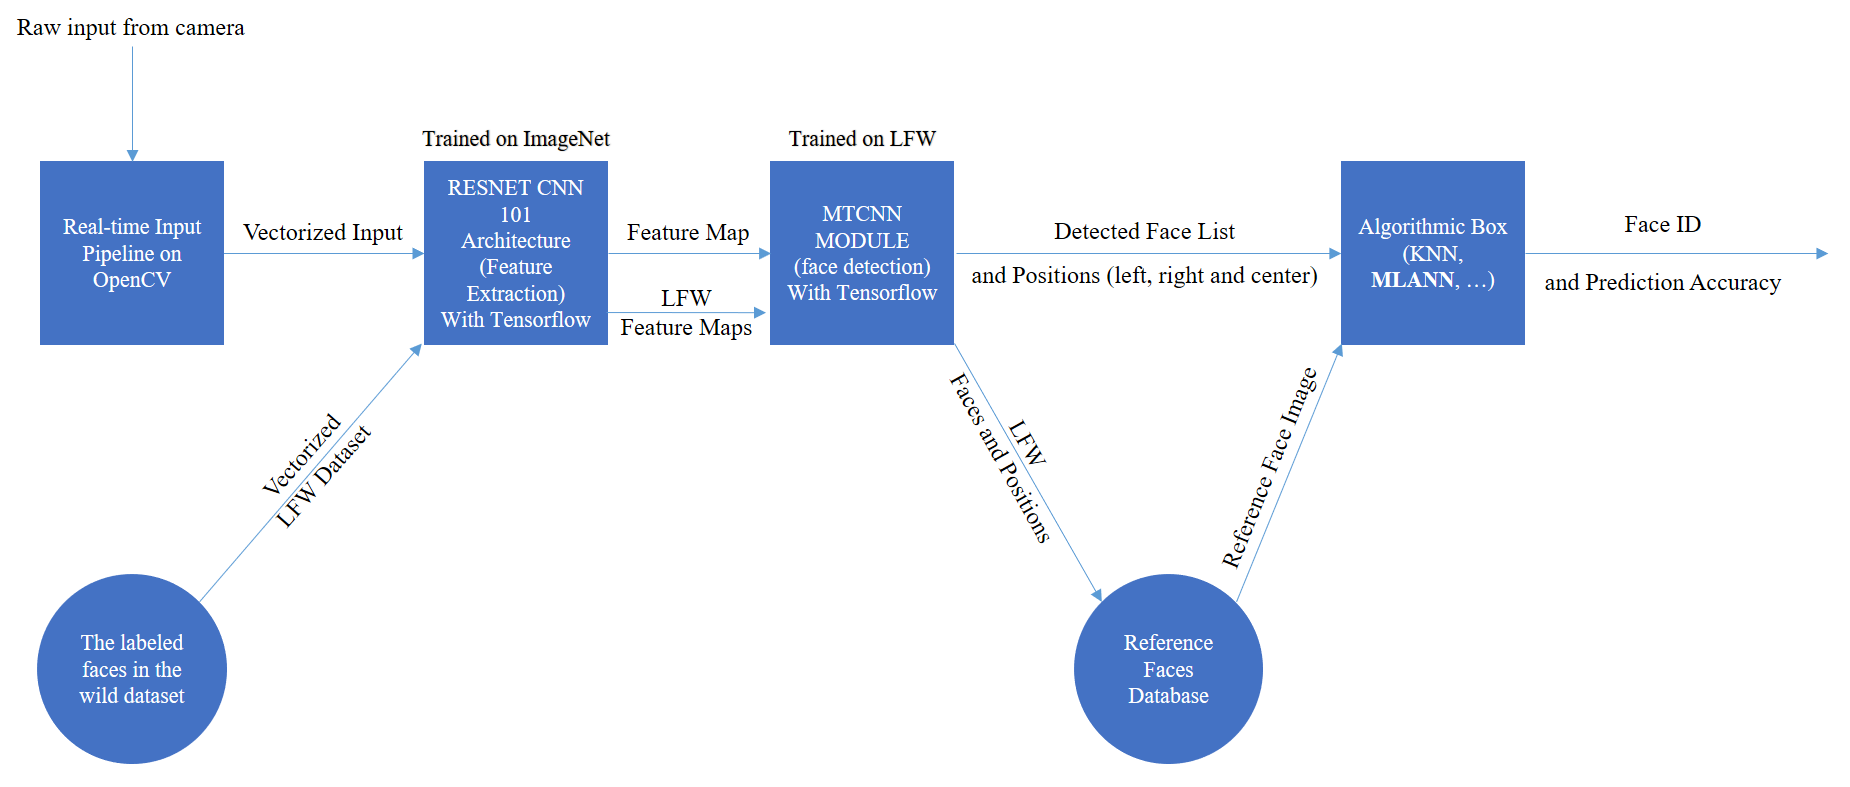
\includegraphics[width=1.1\textwidth]{diagram.PNG}
	\caption{The architecture of real-time face recognition system.}
	\label{pl1}
\end{figure}
\chapter{Future Work}
We admit the possible drawbacks and inefficiencies existing in this project, thus we have the following key improvement to-do list:
\begin{itemize}
	\item Reorganization of the project structure, header files and .c files.
	\item Reorganization of the project source code for a C unified implementation.
	\item Usage shared memory techniques to improve the performance of the \textit{NTM} implementation.
	\item Usage of highly-optimized image libraries such as \textit{OpenCV} for \textit{image rotation}, \textit{image matrix extraction} and general \textit{bitmap processing}.
	\item Implementation of CUDA kernels for real-to-complex signal conversions.
	\item Implementation of CUDA kernel to find the number of occurrences of template signal in main signal in \textit{Fourier} based template matching.
\end{itemize}
\chapter{Conclusion}
In this project, we implemented the novel ANN method by Professor \textit{Savchenko} with the
maximal likelihood search of the next reference instance
in order to improve the performance of the NN-based image
recognition methods. We analyzed its modification P-ML-ANN to
make this approach suitable for practical applications. Several pivots
are chosen at the preprocessing stage of the P-ML-ANN
method. Hence, the main cycle of the search procedure
becomes as fast as the brute force. Although this approach does
not achieve the lowest average number of computed distances as
the ML-ANN, it is more computationally efficient in most cases.
Our modification requires only linear memory space to store the
distances between pivots and all reference images. An obvious
drawback of this procedure is the need for a proper choice of the
number of pivots.e Invariant Feature Transform.
\cleardoublepage
%\pagebreak
\phantomsection
\addcontentsline{toc}{chapter}{References}
\begin{thebibliography}{99}

\bibitem{abstract}Hashemi, Nazanin Sadat, et al. "\textit{Template Matching Advances and Applications in Image Analysis.}" arXiv preprint arXiv:1610.07231 (2016).


\bibitem{intro1}Mahalakshmi, T., R. Muthaiah, and P. Swaminathan. "\textit{An overview of template matching technique in image processing.}" Research Journal of Applied Sciences, Engineering and Technology 4.24 (2012): 5469-5473.

\bibitem{intro2}Perveen, Nazil, Darshan Kumar, and Ishan Bhardwaj. "\textit{An overview on template matching methodologies and its applications.}" IJRCCT 2.10 (2013): 988-995.

\bibitem{intro3}Cox, Greg S. "Template matching and measures of match in image processing." University of Cape Town, South Africa (1995).

\bibitem{amdahl}Andrey Alekseenko (https://stackoverflow.com/users/929437/aland), \textit{Amdahl's law and GPU}, URL (version: 2018-07-13): https://stackoverflow.com/q/12398929.

\bibitem{roofline}Ofenbeck, Georg, et al. "Applying the roofline model." Performance Analysis of Systems and Software (ISPASS), 2014 IEEE International Symposium on. IEEE, 2014.

\bibitem{techpower}Techpowerup (2018, July 14). \textit{NVIDIA GeForce GTX 850M} [On-line]. Available: https://www.techpowerup.com/gpudb/2538/geforce-gtx-850m.

\bibitem{gonzalez}Gonzalez, Rafael C., and Richard E. Woods. "Image processing." Digital image processing 2 (2007).
\end{thebibliography}


\end{document}
